\documentclass[12pt, 
hyperref={colorlinks=true, linkcolor=blue, urlcolor=cyan}]{beamer}
\usetheme{default} 

\setbeamertemplate{navigation symbols}{} %gets rid of navigation symbols
\setbeamertemplate{footline}{} %gets rid of bottom navigation bars
\setbeamertemplate{footline}[page number]{} %use this for page numbers

\setbeamertemplate{itemize items}[circle] %round bullet points
\setlength\parskip{10pt} % white space between paragraphs

\usepackage{comment}
\usepackage{wrapfig}
\usepackage{subfig}
\usepackage{setspace}
\usepackage{enumerate}
\usepackage{graphicx}
\usepackage{amsmath}
\usepackage{amsfonts}
\usepackage{amssymb}
\usepackage{amsthm}
\usepackage[UKenglish]{isodate}
\cleanlookdateon

% the preamble
\title{BIOST 311: \\ Regression Methods for the Health Sciences}
\author{Kelsey Grinde and Brian Williamson}
\institute{UW Biostatistics}
\date{Spring 2018}

\begin{document}
% title slide
\begin{frame}
\titlepage\thispagestyle{empty}
\end{frame}

% make it 2.something
\setbeamertemplate{footline}{%
  \raisebox{5pt}{\makebox[\paperwidth]{\makebox[120pt]{\scriptsize Last updated \today}\hfill\makebox[20pt]{\scriptsize 2.\insertframenumber~~}}}}  \newcounter{chap2}{\value{1}}
\setcounter{framenumber}{\value{chap2}}

\section{Chapter 2 learning objectives}
\begin{frame}
\frametitle{CHAPTER 2: LOGISTIC REGRESSION}

By the end of Chapter 2, you should be able to:
\begin{itemize}
\item Distinguish between probability and odds and know how to calculate each in \texttt{R}
\item Formulate a regression model, given a scientific or statistical question about a binary outcome
\item Interpret the coefficients for a (simple or multiple) linear or logistic regression model with a binary outcome
\item Interpret confidence intervals and p-values for logistic regression coefficients
\item Describe how (and why) logistic regression interpretation changes when we have data from a case-control study
\item Use \texttt{R} to fit a logistic regression model  and to create figures/tables to support your logistic regression analysis
\end{itemize}
\end{frame}

\section{Binary outcomes}
\begin{frame}
\frametitle{SECTION 1: BINARY OUTCOMES}
Up to this point, we've focused on questions involving \textcolor{blue}{quantitative} outcomes:

\begin{itemize}
\item Is lung function (\textcolor{blue}{FEV}) associated with smoking?
\item Is lung function (\textcolor{blue}{FEV}) associated with smoking, after adjusting for age, height, and sex?
\item Does the association between lung function (\textcolor{blue}{FEV}) and smoking, adjusting for age and height, differ between males and females?
\item Is \textcolor{blue}{systolic blood pressure} associated with ancestry?
\item Is cognitive function (\textcolor{blue}{DSST score}) associated with alcohol use, adjusting for age, sex, and education?
\end{itemize}
\end{frame}

% binary outcome examples
\begin{frame}
\frametitle{SECTION 1: BINARY OUTCOMES}
However, we are often interested in questions that involve \textcolor{blue}{binary} outcomes:

\begin{itemize}
\item Are \textcolor{blue}{surgery complications} after upper endoscopy associated with who performed your sedation (anesthesiologist vs nurse)? % my work
\item Is \textcolor{blue}{cervical cancer} associated with hormonal contraceptive use? % group project
\item Is \textcolor{blue}{death from heart disease} associated with smoking?
\item Is \textcolor{blue}{diabetes} associated with sex? with age? % infarcts data
\end{itemize}
\end{frame}

% look at diabetes vs sex example
\begin{frame}
\frametitle{Example: diabetes and sex}

\begin{enumerate}
\item \textbf{Scientific Question:} is diabetes associated with sex?  \pause
\item \textbf{Statistical Question:} what do we mean by \textcolor{orange}{\textit{associated}}?  \pause
\end{enumerate}

There are multiple ways that we could check if diabetes is \textit{associated} with sex... \pause
\begin{itemize}
\item[] $p_M \stackrel{?}{=} p_F$ \textcolor{blue}{(probs)} \quad \quad \quad \quad \pause $\frac{p_M}{1-p_M} \stackrel{?}{=} \frac{p_F}{1-p_F}$ \pause \textcolor{blue}{(odds)} \pause
\item[] $p_M - p_F \stackrel{?}{=} 0$ \pause \textcolor{blue}{(RD)} \pause \quad \quad \quad $\frac{p_M}{1-p_M} - \frac{p_F}{1-p_F} \stackrel{?}{=} 0$ \pause
\item[] $p_M \div p_F \stackrel{?}{=} 1$ \pause \textcolor{blue}{(RR)} \pause \quad \quad \quad  $\left(\frac{p_M}{1-p_M}\right) \div \left(\frac{p_F}{1-p_F}\right) \stackrel{?}{=} 1$ \pause \textcolor{blue}{(OR)}
\end{itemize}
\end{frame}


% defining associations
\begin{frame}
\frametitle{Association}
When figuring out how we want to define \textit{association}, there are two parts that we need to think about...  \vspace{-0.3cm} \pause

\begin{itemize}
\item \textcolor{blue}{Summary measure}: probability, odds, mean
\item \textcolor{orange}{Contrast}: difference, ratio
\end{itemize} \pause

Examples: \vspace{-0.3cm}
\begin{itemize}
\item Is FEV associated with smoking? \pause
	\begin{itemize}
	\item[] $\rightarrow$ Is there a \textcolor{orange}{difference} in \textcolor{blue}{average} FEV between smokers and nonsmokers? \pause
	\end{itemize}
\item Is diabetes associated with sex? \pause
	\begin{itemize}
	\item[] $\rightarrow$ Is there a \textcolor{orange}{difference} in \textcolor{blue}{probability} of diabetes between men and women? \pause
	\item[] $\rightarrow$ Does the \textcolor{orange}{ratio} of \textcolor{blue}{odds} of diabetes between men and women differ from 1? %\pause \begin{tiny}(Note how awkward it is to talk about ratios ``in English")\end{tiny}
	\end{itemize}
\end{itemize}
\end{frame}

\subsection{Simple linear regression with binary outcome}
% diabetes and sex: linear regression
\begin{frame}
\frametitle{Example: diabetes and sex}

\begin{enumerate}
\item \textbf{Scientific Question:} is diabetes \textcolor{orange}{associated} with sex? \pause
\item \textbf{Statistical Question:} is there a \textcolor{orange}{difference in probability} of diabetes between men and women? \pause
	\begin{itemize}
	\item \textbf{Parameter:} difference in probabilities (or \textit{risk difference}) \pause
	\end{itemize}
\item Take a \textbf{sample} from the population: cohort study of adults aged 65 and older from 4 US communities \pause
\item Perform \textit{statistical inference}:
	\begin{itemize}
	\item Calculate a corresponding \textbf{statistic}: difference in probabilities in our sample
	\item Quantify uncertainty in your statistic
	\item Perform a hypothesis test \pause
	\end{itemize}
\end{enumerate}

We can use linear regression to answer this question!
\end{frame}

% aside: mean of a binary variable
\begin{frame}
\frametitle{Linear regression with a binary outcome}

Simple linear regression model: $$E[Y \mid X] = \beta_0 + \beta_1 X$$

$E[Y \mid X]$ is the \textcolor{blue}{\textit{expected value}} of $Y$ given $X$ (or the \textcolor{blue}{\textit{average}}) \pause

What's the average of a binary variable $Y$? \pause \textit{It's the probability that $Y$ equals 1!} $\left(\text{i.e., } E[Y] = \text{P}(Y=1)\right)$ \pause

\begin{itemize} \itemsep +12pt
\item[] $Y = \{ 0, 0, 1, 0, 1, 1, 0, 0, 1, 1 \}$ \pause
\item[] $\bar{Y} = \frac{0 + 0 + 1 + 0 + 1 + 1 + 0 + 0 + 1 + 1}{10} = \frac{1}{2}$ \pause
\item[] $\hat{p} = \widehat{\text{P}(Y=1)} = \frac{5}{10} = \frac{1}{2} $
\end{itemize}
\end{frame}

% activity: interpret lin reg coefficients
\begin{frame}
\frametitle{Activity: diabetes and sex}

Suppose we fit the linear regression model $$E[diabetes \mid male] = \beta_0 + \beta_1 male,$$ \begin{footnotesize}where $diabetes = 1$ if diabetes and $diabetes = 0$ if no diabetes, \\ and $male = 1$ if male and $male = 0$ if female. \end{footnotesize}

\color{blue} On a piece of paper, please answer the following questions: 

\begin{enumerate}
\item \color{blue} Interpret the intercept, $\beta_0$.
\item Interpret the slope, $\beta_1$.
\end{enumerate} \color{black}

(You will turn this in at the end of class.)
\end{frame}

% linear regression: diabetes vs sex
\begin{frame}
\frametitle{Linear regression: diabetes vs sex}

Suppose we fit the linear regression model $$E[diabetes \mid male] = \beta_0 + \beta_1 male$$

How do we interpret the regression coefficients $\beta_0, \beta_1$? \vspace{-0.3cm}

\begin{itemize}
\item \color{blue} $\beta_0$: \pause the probability of diabetes among females \pause \color{black}
\item[] \ \ \begin{scriptsize} (the average value of diabetes among females) \end{scriptsize} \pause
\item \color{blue} $\beta_1$: \pause the difference in probability of diabetes between males and females \pause \color{black}
\item[] \ \ \begin{scriptsize}(the difference in average value of diabetes between males and females) \pause \end{scriptsize}
\end{itemize}

\vspace{-0.3cm}
To answer our statistical question \begin{small}\textit{(is there a difference in probability of diabetes between men and women?)}\end{small} we just need to look at $\beta_1$! \begin{small} (estimate, CI, test if it's equal to 0) \end{small}
\end{frame}

\subsection{Simple logistic regression with binary outcome}
% motivate logistic regression
\begin{frame}
\frametitle{Diabetes vs sex: odds}
\begin{small} What if we wanted to quantify the association between diabetes and sex via the \textit{odds ratio} rather than the \textit{risk difference}? \end{small} \pause

\vspace{-0.3cm}

\begin{enumerate}
\item \textbf{Scientific Question:} is diabetes \textcolor{orange}{associated} with sex? \pause
\item \textbf{Statistical Question:} is the \textcolor{orange}{ratio of odds} of diabetes between men and women different from 1? \pause
	\begin{itemize}
	\item \textbf{Parameter:} odds ratio \pause
	\end{itemize}
\item Take a \textbf{sample} from the population: cohort study of adults aged 65 and older from 4 US communities \pause
\item Perform \textit{statistical inference}:
	\begin{itemize}
	\item Calculate a corresponding \textbf{statistic}: sample odds ratio
	\item Quantify uncertainty in your statistic
	\item Perform a hypothesis test \pause
	\end{itemize}
\end{enumerate}

\vspace{-0.4cm}
We can use \textcolor{blue}{logistic} regression to answer this question!
\end{frame}

% ask them to think about logistic regression interp
\begin{frame}
\frametitle{Activity (continued): diabetes vs sex}
Suppose we fit the logistic regression model $$\log\left(\text{Odds}[diabetes | male]\right) = \beta_0 + \beta_1 male$$

\color{blue} On the same piece of paper, please answer these questions:

\begin{enumerate}
\item[3.] \color{blue} Interpret the intercept, $\beta_0$.
\item[4.] Interpret the slope, $\beta_1$.
\end{enumerate}
\end{frame}

% logistic regression: diabetes vs sex
\begin{frame}
\frametitle{Logistic regression: diabetes vs sex}

Suppose we fit the logistic regression model $$\log\left(\text{Odds}[diabetes | male]\right) = \beta_0 + \beta_1 male$$

\vspace{-0.2cm}

How do we interpret the regression coefficients $\beta_0, \beta_1$? \vspace{-0.3cm}
\begin{itemize}
\item $\beta_0$: \pause the log odds of diabetes among females \pause
\item[] \color{blue} $e^{\beta_0}$: the odds of diabetes among females \pause \color{black}
\item $\beta_1$: \pause the difference in log odds of diabetes between males and females \pause 
\item[] \color{blue} $e^{\beta_1}$: the ratio of odds between males and females \color{black}
\end{itemize}

\vspace{-0.2cm}
To answer our statistical question \begin{small}\textit{(is the ratio of odds of diabetes between men and women different from 1?)}\end{small} we just need to look at $e^{\beta_1}$! \begin{small} (estimate, CI, test if it's equal to 1) \end{small}
\end{frame}

\begin{frame}
The interpretation of logistic regression models is
\begin{itemize}
\item[] \color{blue} more complicated \color{black} (we have to remember to exponentiate the coefficients, and to talk about ratios rather than differences), and
\item[] \color{orange} less intuitive \color{black} (a lot of people don't understand the difference between probabilities and odds)...
\end{itemize}
\textit{so why bother?}
\end{frame}

\section{Linear regression with binary outcomes}
\subsection{Learning objectives}
\begin{frame}
\frametitle{SECTION 2: LINEAR REGRESSION WITH BINARY OUTCOMES}

% Learning objectives
By the end of this section, you should be able to:
\begin{itemize}
\item Interpret linear regression coefficients when the outcome $Y$ is binary
\item Write a summary of results from a linear regression analysis with a binary outcome
\item List at least one advantage and one disadvantage of using linear regression with a binary outcome
\end{itemize}
\end{frame}

\subsection{Simple linear regression interpretation}
\begin{frame}
\frametitle{Simple linear regression with binary outcomes}
% recall activity
Suppose we fit the simple linear regression model $$E[Y \mid X] = \beta_0 + \beta_1 X,$$ where our outcome $Y$ is binary.

\color{orange} Without looking at your notes, \color{black} write down an interpretation for the coefficients in this model.

\begin{enumerate}
\item $\beta_0$
\item $\beta_1$
\end{enumerate} 

(You will turn this in at the end of class.)

\end{frame}

\subsection{Multiple linear regression interpretation}
% interpretation
\begin{frame}
\frametitle{Multiple linear regression with binary outcomes}
Linear regression model with a binary outcome: $$E[Y|X_1,\cdots,X_p] = \beta_0 + \beta_1 X_1 + \beta_2X_2 + \cdots \beta_p X_p$$ $$P[Y=1|X_1,\cdots,X_p] = \beta_0 + \beta_1 X_1 + \beta_2 X_2 + \cdots \beta_p X_p$$

\color{blue} Interpretation: \color{black}
\begin{itemize} 
\item $\beta_0$: \pause probability that $Y=1$ when $X_1 = 0, \cdots X_p = 0$
\item $\beta_1$: \pause difference in probability that $Y=1$ comparing two groups that differ by one unit in $X_1$ but are the same with respect to $X_2,\cdots,X_p$ 
\item ...
\end{itemize}
\end{frame}

\subsection{Statistical Inference}
\begin{frame}
\frametitle{Linear regression with binary outcomes}
\begin{center} $E[Y|X_1,\cdots,X_p] = \beta_0 + \beta_1 X_1 + \beta_2 X_2 + \cdots \beta_p X_p$ \end{center}

\vspace{-0.6cm}
\color{blue} Inference: \vspace{-0.3cm} \color{black}
\begin{itemize}
\item Identify the regression coefficient of interest, $\beta$. \pause % which one(s) answer(s) our scientific Q?
\item Report an estimate of $\beta$, and interpret: \textit{We estimate that the difference in probabilities between two groups...} \pause
\item Report a 95\% confidence interval for $\beta$, and interpret: \textit{Based on a 95\% confidence interval, this observed difference in probabilities would not be judged unusual if...} \pause
\item Report the p-value from a hypothesis test of $H_0: \beta = 0$: \textit{These data provide evidence to suggest that this difference in probabilities is (is not) significantly different from zero ($p =$...).} \pause
\item Add a conclusion relating back to our scientific question
\end{itemize}
% they'll fill in the blanks on HW this week
\end{frame}

\subsection{Prediction}
\begin{frame}
\frametitle{Linear regression with binary outcomes}
\begin{center} $E[Y|X_1,\cdots,X_p] = \beta_0 + \beta_1 X_1 + \beta_2 X_2 + \cdots \beta_p X_p$ \end{center}

\color{blue} Prediction:\vspace{-0.3cm} \color{black}
\begin{itemize} \itemsep +5pt
\item Get estimates for each regression coefficient: $\hat\beta_0, \cdots, \hat\beta_p$ \pause
\item Plug in those estimates, along with the covariate values for the new individual: $\hat\beta_0 + \hat\beta_1 x_1 + \cdots \hat\beta_p x_p$ \pause
	\begin{itemize} \itemsep +5pt
	\item This is our best estimate of $Y$ for a person with $X_1 = x_1, \cdots X_p = x_p$ ($\hat{Y}$) \pause
	\item This is also our estimate of the mean value of $Y$ (or probability that $Y=1$) among subjects with $X_1 = x_1, \cdots, X_p = x_p$ ($\hat{E}[Y|X_1,\cdots X_p] = \hat{P}[Y=1|X]$)
	\end{itemize}
\end{itemize}

\end{frame}

% graphical support: scatterplot
\begin{frame}
\frametitle{Linear regression with binary outcomes}
\begin{center} $E[Y|X_1,\cdots,X_p] = \beta_0 + \beta_1 X_1 + \beta_2 X_2 + \cdots \beta_p X_p$ \end{center}

\color{blue} Graphical support: \color{black} scatterplot
\vspace{-0.55cm}
\center
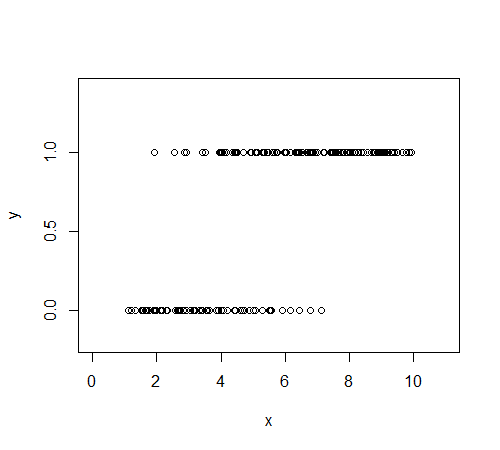
\includegraphics[width=0.7\textwidth]{./figs/scatterplot}
\end{frame}


\begin{frame}[noframenumbering]
\frametitle{Linear regression with binary outcomes}
\begin{center} $E[Y|X_1,\cdots,X_p] = \beta_0 + \beta_1 X_1 + \beta_2 X_2 + \cdots \beta_p X_p$ \end{center}

\color{blue} Graphical support: \color{black} scatterplot + linear regression line
\vspace{-0.55cm}
\center
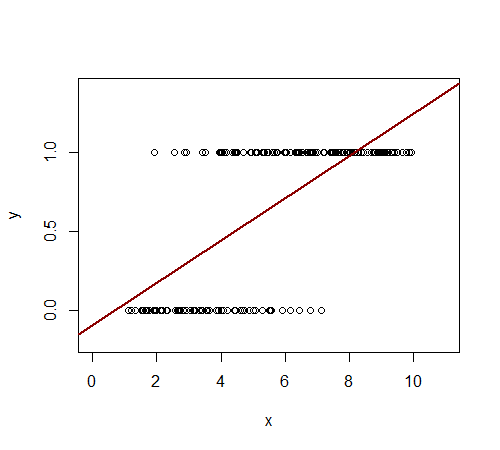
\includegraphics[width=0.7\textwidth]{./figs/scatterplot_lm}
\end{frame}

\begin{frame}[noframenumbering]
\frametitle{Linear regression with binary outcomes}
\begin{center} $E[Y|X_1,\cdots,X_p] = \beta_0 + \beta_1 X_1 + \beta_2 X_2 + \cdots \beta_p X_p$ \end{center}

\color{blue} Graphical support: \color{black} \textit{What is $\hat{Y}$ for someone with $X = 10$?}
\vspace{-0.55cm}
\center
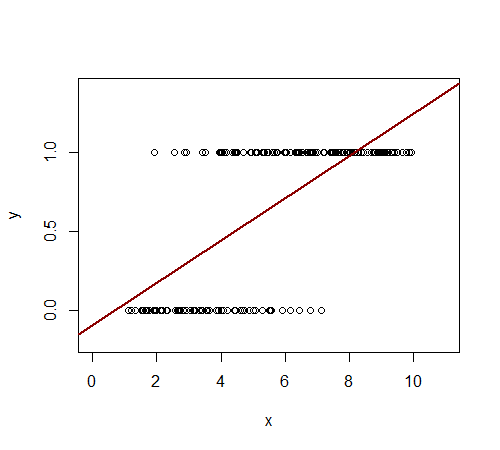
\includegraphics[width=0.7\textwidth]{./figs/scatterplot_lm}
\end{frame}

\subsection{Pros and Cons}
\begin{frame}
\frametitle{Linear regression with binary outcomes}
\begin{center} $E[Y|X_1,\cdots,X_p] = \beta_0 + \beta_1 X_1 + \beta_2 X_2 + \cdots \beta_p X_p$ \end{center}

Pros: \vspace{-0.3cm}
\begin{itemize}
\item Easy to interpret (differences in probabilities)
\end{itemize}

Cons: \vspace{-0.3cm}
\begin{itemize}
\item Predicted/fitted values can be outside the (0,1) range
\item Our mean model might not be correct (particularly the linearity piece)% is one of the assumptions for linear regression that actually is important
\end{itemize}

What can we do instead?
\end{frame}

\section{Logistic regression}
\subsection{Learning objectives}
\begin{frame}
\frametitle{SECTION 3: LOGISTIC REGRESSION}

% Learning objectives
By the end of this section, you should be able to:
\begin{itemize}
\item Interpret regression coefficients for simple and multiple logistic regression models
\item Formulate a logistic regression model given a scientific or statistical question 
\item Use R to fit a logistic regression model and extract relevant results
\item Write a summary of results from a logistic regression analysis
\item Describe the impact of including (or not including) a confounder or precision variable in logistic regression
\item List at least one advantage and one disadvantage of using logistic regression with a binary outcome
\end{itemize}
\end{frame}

\subsection{Simple logistic regression interpretation}
% simple logistic regression recall
\begin{frame}
\frametitle{Simple logistic regression}
Suppose we fit the simple logistic regression model $$\log\left(\text{Odds}[Y =1 \mid X]\right) = \beta_0 + \beta_1 X,$$ where our outcome $Y$ is binary.

\color{orange} Without looking at your notes, \color{black} write down an interpretation for the coefficients in this model.

\begin{enumerate}
\item[3.] $\beta_0$ (and $e^{\beta_0}$)
\item[4.] $\beta_1$  (and $e^{\beta_1}$)
\end{enumerate} 

(You will turn this in at the end of class.)
\end{frame}

\subsection{Multiple logistic regression interpretation}
% interpretation: multiple/general, do the math
%%% beta 0
\begin{frame}
\frametitle{Multiple logistic regression}
$$\log\left(\text{Odds}[Y =1 |X_1,\cdots,X_p]\right) = \beta_0 + \beta_1 X_1 + \beta_2X_2 + \cdots \beta_p X_p$$

\color{blue} Interpretation: \color{black}
% beta0
\begin{itemize}  \color{orange}
\item $\beta_0$: \pause log odds (of $Y=1$) when $X_1 = 0, \cdots, X_p = 0$ \pause
\end{itemize}
\vspace{-0.3cm}
\begin{footnotesize}
\begin{align*}
\log\left(\text{Odds}[Y =1 |X_1=0,\cdots,X_p=0]\right) & = \beta_0 + \beta_1 (0) + \beta_2(0) + \cdots \beta_p (0) \\
& = \beta_0 
\end{align*} \pause
\end{footnotesize}

\vspace{-0.6cm}
%exp(beta0)
\begin{itemize}   \color{orange}
\item $e^{\beta_0}$: \pause odds (of $Y=1$) when $X_1 = 0, \cdots, X_p = 0$ \pause
\end{itemize}
\vspace{-0.3cm}
\begin{footnotesize}
\begin{align*}
e^{\beta_0} & = e^{\log\left(\text{Odds}[Y =1 |X_1=0,\cdots,X_p=0]\right)} \\
& = \text{Odds}[Y =1 |X_1=0,\cdots,X_p=0], \text{ since } \color{blue} e^{log(z)} = z
\end{align*}
\end{footnotesize}

\end{frame}

%%% beta 1
\begin{frame}
\frametitle{Multiple logistic regression}
$$\log\left(\text{Odds}[Y =1 |X_1,\cdots,X_p]\right) = \beta_0 + \beta_1 X_1 + \beta_2X_2 + \cdots \beta_p X_p$$

\color{blue} Interpretation: \color{black}
% beta1
\begin{itemize}  \color{orange}
\item $\beta_1$: difference in log odds (of $Y=1$) comparing two groups that differ by one unit in $X_1$ but are \textbf{the same}\footnote[frame]{Note that we don't have to set $X_2 \cdots X_p$ equal to 0 for this to work!} with respect to $X_2,\cdots,X_p$ \pause
\end{itemize}
\vspace{-0.3cm}
\begin{scriptsize}
\begin{align*}
& \log\left(\text{Odds}[Y =1 |X_1=(x_1+1),X_2=x_2,\cdots,X_p=x_p]\right) \\
& \ \ \ \ \ \ \ \ \ \ - \log\left(\text{Odds}[Y =1 |X_1=(x_1),X_2=x_2,\cdots,X_p=x_p]\right) \\
& \ \ = \left[\beta_0 + \beta_1(x_1+1) + \beta_2 x_2 + \cdots \beta_p x_p\right]\\
& \ \ \ \ \ \ \ \ \ \ - \left[\beta_0 + \beta_1(x_1) + \beta_2 x_2 + \cdots \beta_p x_p\right] \\
& \ \ = \beta_1
\end{align*}
\end{scriptsize}

\end{frame}

%%% exp(beta 1)
\begin{frame}
\frametitle{Multiple logistic regression}
$$\log\left(\text{Odds}[Y =1 |X_1,\cdots,X_p]\right) = \beta_0 + \beta_1 X_1 + \beta_2X_2 + \cdots \beta_p X_p$$

\color{blue} Interpretation: \color{black}
%exp(beta1)
\begin{itemize} \color{orange}
\item $e^{\beta_1}$:  \pause ratio of odds (of $Y=1$) comparing two groups that differ by one unit in $X_1$ but are \textbf{the same} with respect to $X_2,\cdots,X_p$  \pause 
\end{itemize}
\vspace{-0.3cm}
\begin{scriptsize}
\begin{align*}
\beta_1 & = \log\left(\text{Odds}[Y =1 |X_1=(x_1+1),X_2=x_2,\cdots,X_p=x_p]\right) \\
& \ \ \ \ \ \ \  - \log\left(\text{Odds}[Y =1 |X_1=(x_1),X_2=x_2,\cdots,X_p=x_p]\right) \\
& = \log\left(\frac{\text{Odds}[Y =1 |X_1=(x_1+1),X_2=x_2,\cdots,X_p=x_p]}{\text{Odds}[Y =1 |X_1=(x_1),X_2=x_2,\cdots,X_p=x_p]} \right) \color{blue} \left[ \log(a)-\log(b) = \log\left(\frac{a}{b}\right)\right] \\
e^{\beta_1} & = \frac{\text{Odds}[Y =1 |X_1=(x_1+1),X_2=x_2,\cdots,X_p=x_p]}{\text{Odds}[Y =1 |X_1=(x_1),X_2=x_2,\cdots,X_p=x_p]} \color{blue} \left[e^{\log(z)} = z\right]
\end{align*}
\end{scriptsize}

\end{frame}

% interpretation: pull it back together
\begin{frame}
\frametitle{Multiple logistic regression}
$$\log\left(\text{Odds}[Y =1 |X_1,\cdots,X_p]\right) = \beta_0 + \beta_1 X_1 + \beta_2X_2 + \cdots \beta_p X_p$$

\color{blue} Interpretation: \color{black}
\begin{itemize}
\item $\beta_0$:  log odds (of $Y=1$) when $X_1 = 0, \cdots, X_p = 0$
\item \color{orange} $e^{\beta_0}$: \pause odds (of $Y=1$) when $X_1 = 0, \cdots, X_p = 0$ \color{black} \pause
\item $\beta_1$: difference in log odds (of $Y=1$) comparing two groups that differ by one unit in $X_1$ but are the same with respect to $X_2,\cdots,X_p$ \pause
\item \color{orange} $e^{\beta_1}$: \pause ratio of odds (of $Y=1$) comparing two groups that differ by one unit in $X_1$ but are the same with respect to $X_2,\cdots,X_p$ \color{black}
\end{itemize}

\end{frame}

\subsection{Connection to linear regression with log-transformed outcome}
% interpretation: relate back to log(Y) interp
%%% beta 0
\begin{frame}
\frametitle{Recall: $\log(Y)$ in linear regression}
$$E[\log(Y)|X] = \beta_0 + \beta_1 X$$

\color{blue} Interpretation: \color{black}
\begin{itemize} 
\item $\beta_0$: \textcolor{orange}{average} \textcolor{blue}{log} $Y$ among subjects with $X = 0$
	\begin{itemize}
	\item[] $\color{orange}E[ \color{blue}\log(\color{black}Y\color{blue})\color{black}|X=0\color{orange}]$
	\end{itemize} \pause
\item $\beta_0$: \textcolor{blue}{log} \textcolor{orange}{geometric mean} of $Y$ among subjects with $X = 0$
	\begin{itemize}
	\item[] $\color{blue}\log\left(\color{orange} e^{E[\log(Y)\color{black}|X=0\color{orange}]}\color{blue}\right) \color{black} = E[\log(Y)|X=0]$
	\end{itemize} \pause
\item $e^{\beta_0}$: geometric mean of $Y$ among subjects with $X = 0$
\end{itemize}
\end{frame}

% interpretation: relate back to log(Y) interp
%%% beta 1
\begin{frame}
\frametitle{Recall: $\log(Y)$ in linear regression}
$$E[\log(Y)|X] = \beta_0 + \beta_1 X$$
\color{blue} Interpretation: \color{black} \vspace{-0.3cm}
\begin{itemize} 
\item $\beta_1$: \textcolor{gray}{difference} in \textcolor{orange}{average} \textcolor{blue}{log} $Y$ comparing 2 groups of subjects that differ by 1 unit in $X$
	\begin{itemize}
	\item[] $\color{orange}E[ \color{blue}\log(\color{black}Y\color{blue})\color{black}|X=x+1\color{orange}] \color{gray} - \color{orange}E[ \color{blue}\log(\color{black}Y\color{blue})\color{black}|X=x\color{orange}] $
	\end{itemize} \pause
\item $\beta_1$: \textcolor{gray}{difference} in \textcolor{blue}{log} \textcolor{orange}{geometric mean} of $Y$ comparing 2 groups of subjects that differ by 1 unit in $X$
	\begin{itemize}
	\item[] $\color{blue}\log\left(\color{orange} e^{E[\log(Y)\color{black}|X=x+1\color{orange}]}\color{blue}\right) \color{gray} - \color{blue}\log\left(\color{orange} e^{E[\log(Y)\color{black}|X=x\color{orange}]}\color{blue}\right) $
	\end{itemize} \pause
\item $\beta_1$: \textcolor{blue}{log} of \textcolor{gray}{ratio} of \textcolor{orange}{geometric means} of $Y$ comparing 2 groups of subjects that differ by 1 unit in $X$
	\begin{itemize}
	\item $\color{blue}\log\left(\color{orange} e^{E[\log(Y)\color{black}|X=x+1\color{orange}]} \color{gray} \div \color{orange} e^{E[\log(Y)\color{black}|X=x\color{orange}]} \color{blue} \right)$
	\end{itemize} \pause
\item $e^{\beta_1}$: ratio of geometric means of $Y$ comparing 2 groups of subjects that differ by 1 unit in $X$
\end{itemize}
\end{frame}

% interpretation: relate back to log(Y) interp
%%% tying it all together
\begin{frame}
\frametitle{Tying it all together}

\textcolor{orange}{Simple linear regression with log-transformed $Y$:} \begin{small}$$E[\log(Y)|X] = \beta_0 + \beta_1 X$$\end{small} \vspace{-0.8cm}
\begin{itemize}
\item $e^{\beta_0}$: \textcolor{orange}{geometric mean of $Y$} among subjects with $X = 0$
\item $e^{\beta_1}$: \textcolor{orange}{ratio of geometric means of $Y$} comparing 2 groups of subjects that differ by 1 unit in $X$
\end{itemize}

\textcolor{blue}{Simple logistic regression with binary $Y$:} \begin{small}$$\log\left(\text{Odds}[Y=1|X]\right) = \beta_0 + \beta_1 X$$ \end{small}\vspace{-0.8cm}
\begin{itemize}
\item $e^{\beta_0}$: \textcolor{blue}{odds of $Y=1$} among subjects with $X = 0$
\item $e^{\beta_1}$: \textcolor{blue}{ratio of odds of $Y=1$} comparing 2 groups of subjects that differ by 1 unit in $X$
\end{itemize}

\end{frame}

\subsection{Formulating a logistic regression model}
% formulating regression model from scientific question: example with endoscopy dataset
\begin{frame}
\frametitle{Low birth weight: study design}

We will analyze data from a cohort study conducted in a transitional rural/urban setting in the Western Cape, South Africa. 

The study followed 755 pregnant women with singleton pregnancies who could not afford private healthcare from enrollment (on average at 22 weeks gestation) to delivery. 

We have information about each mother (height (cm), age at enrollment (years), number or prior deliveries, smoking status) and her baby (birth weight, sex, gestational age (weeks) at delivery).

\textbf{We are interested in assessing the potential association between maternal smoking and infant birth weight.}
\end{frame}

\begin{frame}
\frametitle{Low birth weight: formulating a statistical question}
\begin{enumerate}
\item \textbf{Scientific Question:} is \textcolor{blue}{infant birth weight} \textcolor{orange}{associated} with maternal smoking?
\item \textbf{Statistical Question:} 
	\begin{itemize}
	\item How are we going to quantify our outcome?
	\item[]
	\item How will we quantify association?
	\item[]
	\item Are there other variables we need to adjust for?
	\item[]
	\end{itemize}
\end{enumerate}

\end{frame}

\begin{frame}[noframenumbering]
\frametitle{Low birth weight: formulating a statistical question}
\begin{enumerate}
\item \textbf{Scientific Question:} is \textcolor{blue}{infant birth weight} \textcolor{orange}{associated} with maternal smoking?
\item \textbf{Statistical Question:} 
	\begin{itemize}
	\item How are we going to quantify our outcome?
	\item[] \textcolor{blue}{Low birth weight (1: $<$ 2500g, 0: $\ge$ 2500 g)}
	\item How will we quantify association?
	\item[]
	\item Are there other variables we need to adjust for?
	\item[]
	\end{itemize}
\end{enumerate}
\end{frame}

\begin{frame}[noframenumbering]
\frametitle{Low birth weight: formulating a statistical question}
\begin{enumerate}
\item \textbf{Scientific Question:} is \textcolor{blue}{infant birth weight} \textcolor{orange}{associated} with maternal smoking?
\item \textbf{Statistical Question:} 
	\begin{itemize}
	\item How are we going to quantify our outcome?
	\item[] \textcolor{blue}{Low birth weight (1: $<$ 2500g, 0: $\ge$ 2500 g)}
	\item How will we quantify association?
	\item[] \textcolor{orange}{Ratio of odds of low birth weight (LBW)}
	\item Are there other variables we need to adjust for?
	\item[]
	\end{itemize}
\end{enumerate}
\end{frame}

\begin{frame}[noframenumbering]
\frametitle{Low birth weight: formulating a statistical question}
\begin{enumerate}
\item \textbf{Scientific Question:} is \textcolor{blue}{infant birth weight} \textcolor{orange}{associated} with maternal smoking?
\item \textbf{Statistical Question:} 
	\begin{itemize}
	\item How are we going to quantify our outcome?
	\item[] \textcolor{blue}{Low birth weight (1: $<$ 2500g, 0: $\ge$ 2500 g)}
	\item How will we quantify association?
	\item[] \textcolor{orange}{Ratio of odds of low birth weight (LBW)}
	\item Are there other variables we need to adjust for?
	\item[] \textcolor{orange}{Let's draw the causal diagram!} \pause
	\end{itemize}
\end{enumerate}

Is the \textcolor{orange}{ratio of odds} of delivering a \textcolor{blue}{LBW} baby \textcolor{orange}{different from 1,} comparing smoking mothers to nonsmoking mothers \textcolor{orange}{with the same age, height, number of prior deliveries, and sex of their baby}?

\end{frame}

% write out model
\begin{frame}
\frametitle{Low birth weight: writing the regression model}

\begin{enumerate}
\item \textbf{Scientific Question:} is infant birth weight associated with maternal smoking? \pause
\item \textbf{Statistical Question:} is the ratio of odds of delivering a LBW baby different from 1, comparing smoking mothers to nonsmoking mothers with the same age, height, number of prior deliveries, and sex of their baby? \pause
\end{enumerate}

\textbf{Regression Model:}
\begin{align*}
\log & \left(\text{Odds}[ \text{LBW} \mid \text{mSmoker, mAge, mHeight, mDeliv, iMale}]\right) \\
& = \beta_0 + \beta_1 \text{mSmoker} + \beta_2 \text{mAge} + \beta_3 \text{mHeight} \\
& \hspace{1cm} + \beta_4 \text{mDeliv} + \beta_5 \text{iMale}
\end{align*}

\end{frame}

\subsection{Fitting logistic regression in R}
\begin{frame}
\frametitle{Low birth weight: fitting our model in \texttt{R}}
Just like with linear regression, we can use the \texttt{regress()} function in the \texttt{uwIntroStats} package to fit logistic regression models!

We only have to change one argument: \texttt{`mean'} $\rightarrow$ \texttt{`odds'}.

Everything else is the same!
\end{frame}

\begin{frame}
\frametitle{Low birth weight: fitting our model in \texttt{R}}
% fitting in R: example with pregnancy dataset
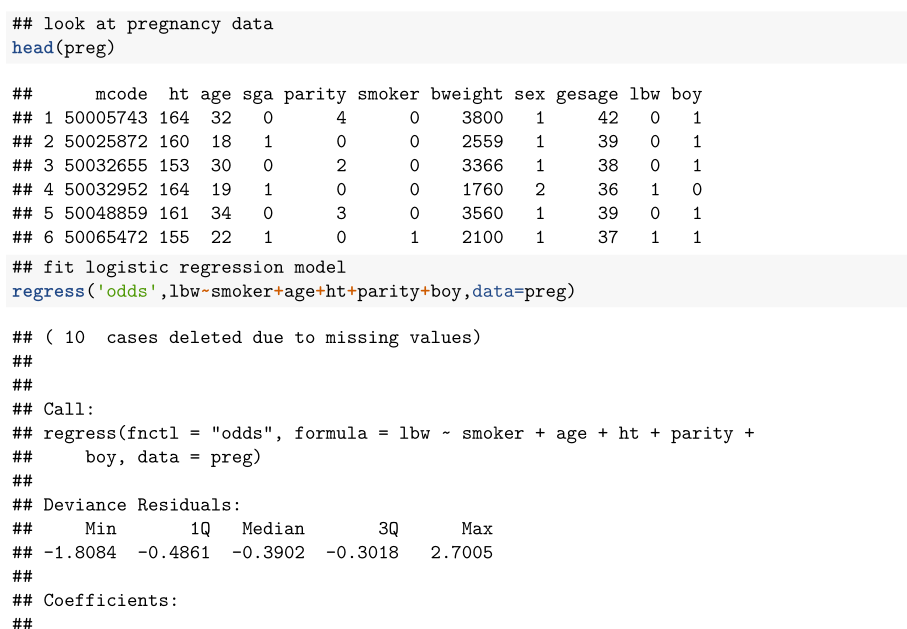
\includegraphics[width=\textwidth]{./figs/pregnancy_head}
\end{frame}

\begin{frame}
% fitting in R: example with pregnancy dataset
\vspace{0.1cm}
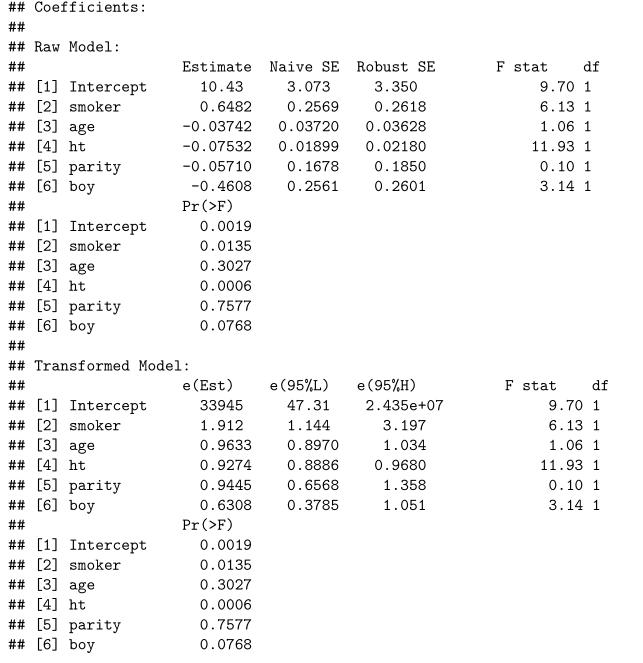
\includegraphics[width=0.82\textwidth]{./figs/pregnancy_coef}
\end{frame}

% highlight raw coef
\begin{frame}[noframenumbering]
% which #s do we care about?
\vspace{0.1cm}
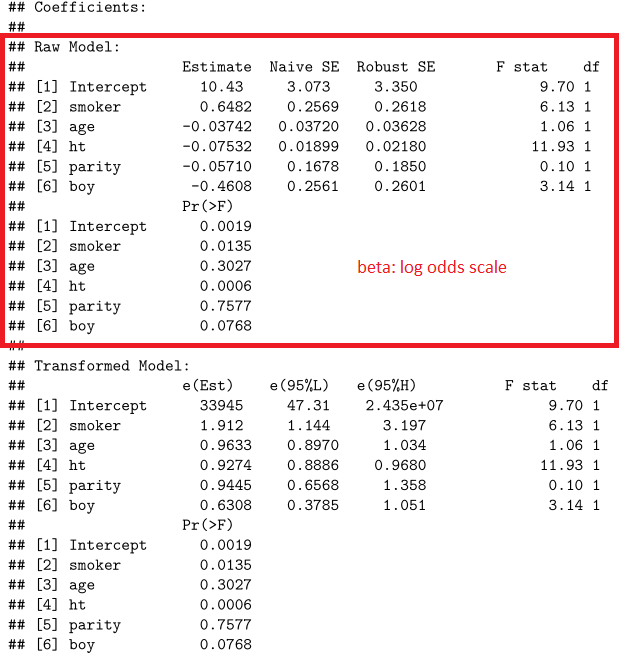
\includegraphics[width=0.82\textwidth]{./figs/pregnancy_coef_raw}
\end{frame}

% highlight transformed coef
\begin{frame}[noframenumbering]
% which #s do we care about?
\vspace{0.1cm}
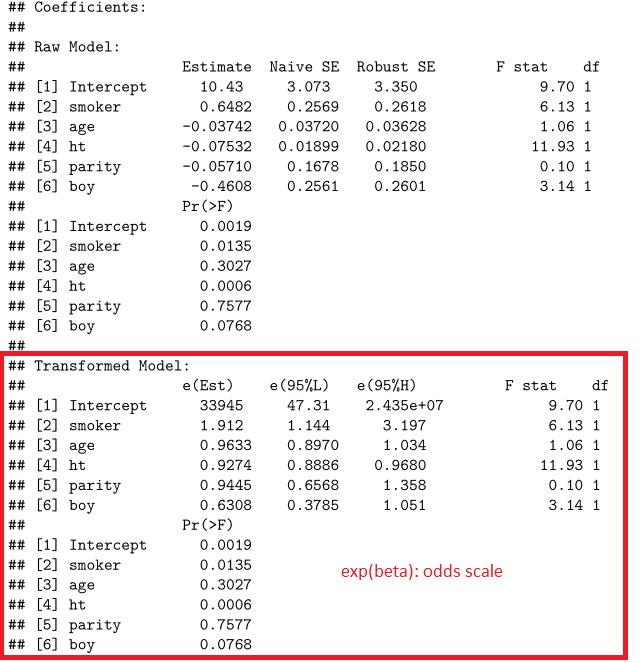
\includegraphics[width=0.82\textwidth]{./figs/pregnancy_coef_exp}
\end{frame}

\subsection{Reporting logistic regression results}
% inference: example with pregnancy dataset (they do this as activity)
\begin{frame}
\frametitle{Low birth weight: reporting results}
\textbf{Scientific Question:} is infant birth weight associated with maternal smoking? 

\textbf{Regression Model:}
$\log \left(\text{Odds}[ \text{LBW} \mid \text{mSmoker, mAge, mHeight, mDeliv, iMale}]\right) = \beta_0 + \beta_1 \text{mSmoker} + \beta_2 \text{mAge} + \beta_3 \text{mHeight} + \beta_4 \text{mDeliv} + \beta_5 \text{iMale}$

\color{blue} Inference: \color{black}
\begin{enumerate}
\item Identify the regression coefficient(s) of interest.
\item Report an estimate, and interpret.
\item Report a 95\% confidence interval, and interpret.
\item Report a p-value, and interpret. 
\item Add a conclusion relating back to our scientific question.
\end{enumerate}

% activity: jigsaw this?
\end{frame}


\begin{frame}[noframenumbering]
\frametitle{Low birth weight: reporting results}
\textbf{Scientific Question:} is infant birth weight associated with maternal smoking? 

\textbf{Regression Model:}
$\log \left(\text{Odds}[ \text{LBW} \mid \text{mSmoker, mAge, mHeight, mDeliv, iMale}]\right) = \beta_0 + \beta_1 \text{mSmoker} + \beta_2 \text{mAge} + \beta_3 \text{mHeight} + \beta_4 \text{mDeliv} + \beta_5 \text{iMale}$

\color{blue} Inference: \color{black}
\begin{enumerate}
\item Identify the regression coefficient(s) of interest: \color{blue} $e^{\beta_1}$ \color{black}
\item Report an estimate, and interpret.
\item Report a 95\% confidence interval, and interpret.
\item Report a p-value, and interpret. 
\item Add a conclusion relating back to our scientific question.
\end{enumerate}
\end{frame}


% hide this before class
%\begin{comment}
\begin{frame}
\frametitle{Low birth weight: reporting results}
\textit{2. Report an estimate and interpret.}

Based on logistic regression, we estimate that the \textcolor{orange}{ratio of odds} of delivering a LBW baby, comparing smoking mothers to nonsmoking mothers with the same age, height, number of previous deliveries, and sex of their baby, \textcolor{orange}{is  1.91}, where the smoking mothers have a higher odds of delivering a LBW baby. \pause

\textbf{Option 2:} Based on logistic regression, we estimate that \textcolor{orange}{the odds} of delivering a LBW baby \textcolor{orange}{is 91\% higher} for smoking mothers than for nonsmoking mothers with the same... \pause

\textbf{Option 3:} Based on logistic regression, we estimate that \textcolor{orange}{the odds} of delivering a LBW baby for smoking mothers \textcolor{orange}{is 1.91 times} that for nonsmoking mothers with the same...

\end{frame}

% CI
\begin{frame}
\frametitle{Low birth weight: reporting results}
\textit{3. Report a 95\% confidence interval, and interpret.}

Based on a 95\% confidence interval, this estimate would not be judged unusual if the true odds ratio were between 1.14 and 3.20. \pause

\textit{4. Report a p-value, and interpret.}

These data provide evidence to suggest that this odds ratio is statistically significantly different from one (p = 0.014). \pause

\textit{5. Add a conclusion relating back to our scientific question.}

Based on these results, we have evidence to suggest that the odds of delivering a LBW baby is associated with maternal smoking, after adjusting for maternal age, height, and number of previous deliveries, and infant sex.

\end{frame}
%\end{comment}


\subsection{Prediction}
\begin{frame}
\frametitle{Prediction}
We can also use logistic regression for prediction. $$\log\left(\text{Odds}[\text{Diabetes}| \text{BMI}]\right) = \beta_0 + \beta_1 \text{BMI}$$

Let's predict for a person with \textcolor{orange}{BMI = 30 kg/m$^2$}:

\begin{enumerate}
\item Get estimates for each regression coefficient: $\hat\beta_0 = -4.363, \hat\beta_1 = 0.099$
\item Plug in the estimates and the covariate values: \pause
	\begin{itemize}
	\item[a.] $\widehat{\log(\text{Odds})} = -4.363 +  0.099\color{orange}(30)\color{black} = -1.393$ \pause
	\item[b.] $\widehat{\text{Odds}} = e^{-1.393} = 0.248$, \color{blue} since $o = e^{\log(o)}$ \color{black} \pause
	\item[c.] $\widehat{\text{Prob}} = 0.248/(1+0.248) = 0.199$, \color{blue} since $p = o/(1+o)$ \color{black} \pause
	\item[] $\widehat{\text{Prob}} = \text{expit}(-1.393) = e^{-1.393}/(1+e^{-1.393})= 0.199$
	\end{itemize}
\end{enumerate}
\end{frame}

% example 2
\begin{frame}
\frametitle{Prediction}
We can also use logistic regression for prediction. $$\log\left(\text{Odds}[\text{Diabetes}| \text{BMI}]\right) = \beta_0 + \beta_1\text{BMI}$$

Let's predict for a person with \textcolor{violet}{BMI = 15 kg/m$^2$}:

\begin{enumerate}
\item Get estimates for each regression coefficient: $\hat\beta_0 = -4.363, \hat\beta_1 = 0.099$
\item Plug in the estimates and the covariate values:
	\begin{itemize}
	\item[a.] $\widehat{\log(\text{Odds})} = -4.363 + 0.099\color{violet}(15) \color{black} = -2.878$
	\item[b.] $\widehat{\text{Odds}} = e^{-2.878} = 0.056$
	\item[c.] $\widehat{\text{Prob}} = \text{expit}(-2.878) = e^{-2.878}/(1+e^{-2.878})= 0.053$
	\end{itemize}
\end{enumerate}
\end{frame}

\begin{frame}
\frametitle{Prediction}

We can also let \texttt{R} do all the work for us:

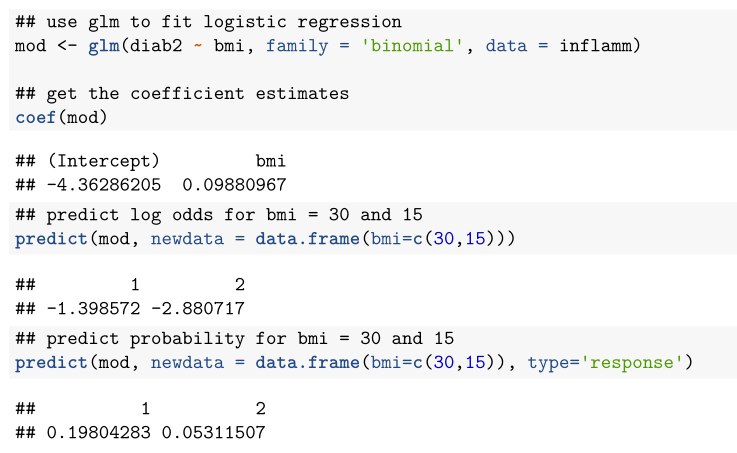
\includegraphics[width=\textwidth]{figs/inflamm_predict}
\pause
\begin{scriptsize}
\textcolor{orange}{(Remember, our linear regression predictions from HW5 were 0.209 and -0.010.)}
\end{scriptsize}

\end{frame}


% prediction: show that it keeps things between 0 and 1
\begin{frame}
\frametitle{Prediction}
\begin{footnotesize}
Linear regression fitted and predicted values can be outside [0,1]:\end{footnotesize}
\vspace{-0.55cm}
\center
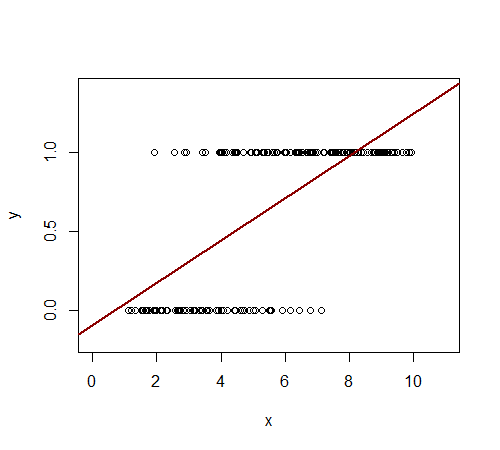
\includegraphics[width=0.8\textwidth]{figs/scatterplot_lm}
\end{frame}

\begin{frame}
\frametitle{Prediction}
\begin{footnotesize}Logistic regression keeps all fitted and predicted values in [0,1]\end{footnotesize}
\vspace{-0.55cm}
\center
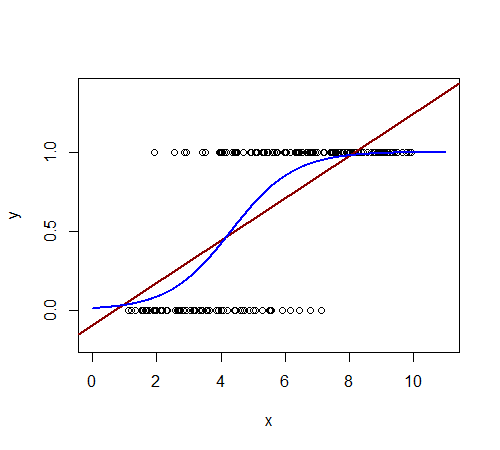
\includegraphics[width=0.8\textwidth]{figs/scatterplot_logit}
\end{frame}


\subsection{Pros and Cons}
\begin{frame}
\frametitle{Logistic regression: pros and cons}
% summary: pros (stay in [0,1]) and cons (less intuitive/harder to interpret)
\begin{center} $\log\left(\text{Odds}[Y=1|X_1,\cdots,X_p]\right) = \beta_0 + \beta_1 X_1 + \beta_2 X_2 + \cdots \beta_p X_p$ \end{center}

Pros: \vspace{-0.3cm}
\begin{itemize}
\item Predicted/fitted values will stay inside the [0,1] range
\item Useful for case-control studies (we'll come back to this)
\end{itemize}

Cons: \vspace{-0.3cm}
\begin{itemize}
\item Harder to interpret (odds, ratios) 
\end{itemize}

\end{frame}


\section{Generalized linear models}
\begin{frame}
\frametitle{SECTION 4: GENERALIZED LINEAR MODELS}

Linear regression and logistic regression are two examples of a larger class of models called \textit{generalized linear models} (GLMs)\footnote[frame]{This is why the \texttt{R} function we use for logistic regression is called \texttt{glm}}.
$$g\left(E[Y|X_1,\cdots,X_p]\right) = \beta_0 + \beta_1 X_1 + \cdots \beta_pX_p$$ \pause

% general formulation
\vspace{-0.2cm}
\begin{itemize}
\item \textbf{Linear regression:} $g(x) = x$ $$E[Y|X_1,\cdots,X_p] = \beta_0 + \beta_1 X_1 + \cdots \beta_pX_p$$ \pause
\item \textbf{Logistic regression:} $g(x) = \text{logit}(x) = \log(\frac{x}{1-x})$ $$\log\left(\frac{E[Y|X_1,\cdots,X_p]}{1-E[Y|X_1,\cdots,X_p]}\right) = \beta_0 + \beta_1 X_1 + \cdots \beta_pX_p$$
\end{itemize}


\end{frame}

\begin{frame}
\frametitle{Relative risk regression}

Another useful type of GLM is \textit{Poisson regression}, also known as \textit{relative risk regression} in the context of binary outcomes.

Here, $g(x) = \log(x)$, so the regression model takes the form $$\log\left(E[Y|X_1,\cdots,X_p]\right) = \beta_0 + \beta_1 X_1 + \cdots \beta_pX_p$$ \pause

When $Y$ is binary, this is the same as $$\log\left(\text{Prob}[Y=1|X_1,\cdots,X_p]\right) = \beta_0 + \beta_1 X_1 + \cdots \beta_pX_p$$ \pause

\vspace{-0.1cm}
Interpretation:\vspace{-0.3cm}
\begin{itemize}
\item $e^{\beta_0}$: probability that $Y=1$ when $X_1 = \cdots X_p = 0$ \pause
\item $e^{\beta_1}$: relative risk (of $Y=1$) comparing 2 groups that differ by 1 unit in $X_1$ but have the same $X_2, \cdots, X_p$
\end{itemize} 

% do the math on the board if time
\end{frame}


\begin{frame}
\frametitle{Relative risk regression}

To fit a relative risk regression model in \texttt{R} you have two options:

\begin{itemize}
\item \texttt{regress(`rate', y $\sim$ x, data = dat)}
	\begin{itemize}
	\item Uses robust standard errors by default
	\end{itemize}
\item \texttt{glm(y $\sim$ x, family = `poisson', data = dat)}
	\begin{itemize}
	\item Uses naive standard errors by default
	\item Can be easier to use for prediction
	\end{itemize}
\end{itemize}

% will keep probabilities positive, but not necessarily constrained to be less than 1?

\end{frame}

\section{Summary of regression methods for binary outcomes}
\begin{frame}
\frametitle{SECTION 5: SUMMARY}
%% summary: come back to slide 2.4 and highlight which type of regression answers which statistical question

\textit{Let's go back to slide 2.4 at the start of this chapter:}

There are multiple ways that we could check if diabetes is \textit{associated} with sex... 
\begin{itemize}
\item[] $p_M \stackrel{?}{=} p_F$ \textcolor{blue}{(probs)} \quad \quad \quad \quad  $\frac{p_M}{1-p_M} \stackrel{?}{=} \frac{p_F}{1-p_F}$ \textcolor{blue}{(odds)} 
\item[]
\item[] $p_M - p_F \stackrel{?}{=} 0$  \textcolor{blue}{(RD)}  \quad \quad \quad $\frac{p_M}{1-p_M} - \frac{p_F}{1-p_F} \stackrel{?}{=} 0$ 
\item[]
\item[] $p_M \div p_F \stackrel{?}{=} 1$  \textcolor{blue}{(RR)}  \quad \quad \quad  $\left(\frac{p_M}{1-p_M}\right) \div \left(\frac{p_F}{1-p_F}\right) \stackrel{?}{=} 1$ \textcolor{blue}{(OR)}
\item[]
\end{itemize} 
\textit{What types of regression answer which questions?}

\end{frame}

\begin{frame}[noframenumbering]
\frametitle{SECTION 5: SUMMARY}

\textit{Let's go back to slide 2.4 at the start of this chapter:}

There are multiple ways that we could check if diabetes is \textit{associated} with sex... 
\begin{itemize}
\item[] $p_M \stackrel{?}{=} p_F$ \textcolor{blue}{(probs)} \quad \quad \quad \quad  $\frac{p_M}{1-p_M} \stackrel{?}{=} \frac{p_F}{1-p_F}$ \textcolor{blue}{(odds)} 
\item[] 
\item[] $p_M - p_F \stackrel{?}{=} 0$  \textcolor{blue}{(RD)}  \quad \quad \quad $\frac{p_M}{1-p_M} - \frac{p_F}{1-p_F} \stackrel{?}{=} 0$ 
\item[] \textcolor{orange}{Linear Regression}
\item[] $p_M \div p_F \stackrel{?}{=} 1$  \textcolor{blue}{(RR)}  \quad \quad \quad  $\left(\frac{p_M}{1-p_M}\right) \div \left(\frac{p_F}{1-p_F}\right) \stackrel{?}{=} 1$ \textcolor{blue}{(OR)}
\item[] \textcolor{orange}{Poisson Regression} \quad \quad \quad \textcolor{orange}{Logistic Regression}
\end{itemize} 
\textit{What types of regression answer which questions?}

\end{frame}


\section{Case-control studies}
\begin{frame}
\frametitle{SECTION 6: LOGISTIC REGRESSION IN CASE-CONTROL STUDIES}

How we've collected our data impacts the way we can interpret our results:

\begin{itemize}
\item \textcolor{blue}{Example:} Experimental vs observational study (causation vs association)
\item \textcolor{blue}{New example:} case-control studies
\end{itemize}

\end{frame}


% case-control studies slide from Chapter 0
\begin{frame}
\frametitle{Case-control studies (Slide 0.12)}
Description: \vspace{-0.3cm}
\begin{itemize}
\item \textit{Sample individuals based on the outcome} (some with, some without), look back in time (usually) for exposure % when you look back in time = retrospective case-control study
\end{itemize}

Pros:\vspace{-0.3cm}
\begin{itemize}
\item Efficient for rare diseases % (don't have to recruit as many people)
\item Cheaper and faster than cohort studies
\item Can study multiple exposures
\end{itemize}

Cons:\vspace{-0.3cm}
\begin{itemize}
%\item Recall bias
\item May not know time sequence of disease and exposure
\item Cannot use to estimate relative risk or disease prevalence
\item Potential confounding (so no conclusions about causality)
\end{itemize}
\end{frame}

\begin{frame}[noframenumbering]
\frametitle{Case-control studies (Slide 0.12)}
Description: \vspace{-0.3cm}
\begin{itemize}
\item \textit{Sample individuals based on the outcome} (some with, some without), look back in time (usually) for exposure % when you look back in time = retrospective case-control study
\end{itemize}

Pros:\vspace{-0.3cm}
\begin{itemize}
\item Efficient for rare diseases % (don't have to recruit as many people)
\item Cheaper and faster than cohort studies
\item Can study multiple exposures
\end{itemize}

Cons:\vspace{-0.3cm}
\begin{itemize}
%\item Recall bias
\item May not know time sequence of disease and exposure
\item \textcolor{orange}{Cannot use to estimate relative risk or disease prevalence}
\item Potential confounding (so no conclusions about causality)
\end{itemize}
\end{frame}

\begin{frame}
\frametitle{Why not?}

In case-control studies, we cannot estimate the relative risk or disease prevalence.

Why not? 
\begin{itemize}
\item This is a biased sampling scheme 
\item Rather than a representative ``random" sample of the population, you are purposely sampling more individuals who have the outcome ($Y = 1$) than you would get from a random sample 
\item Within the categories $Y = 1$ and $Y = 0$, the samples should still be random ; but \textit{overall}, the sample is not 
\end{itemize}

\end{frame}

% cannot estimate prevalence or RR
\begin{frame}
\frametitle{$2 \times 2$ Table}
\begin{center}
\begin{table}
	\begin{tabular}{|c|cc|c|}
	\hline 
	& Lung Cancer & No Lung Cancer &  \\ 
	& (Case) & (Control) & Total  \\
	\hline 
	Smoke & 30 & 5  & 35 \\ 
	No Smoke & 70 & 95 & 165  \\ 
	\hline 
	Total & 100 & 100 & 200 \\ 
	\hline 
	\end{tabular}
\end{table}
\end{center}
\begin{align*} 
P(\text{Cancer}|\text{Smoker}) &\overset{?}{=} \frac{30}{35} \\ 
P(\text{Cancer}|\text{Nonsmoker}) &\overset{?}{=} \frac{70}{165} \\ 
\end{align*} % NO!!
\end{frame}

% can look in other direction
\begin{frame}
\frametitle{$2 \times 2$ Table}
\begin{center}
\begin{table}
	\begin{tabular}{|c|cc|c|}
	\hline 
	& Lung Cancer & No Lung Cancer &  \\ 
	& (Case) & (Control) & Total  \\
	\hline 
	Smoke & 30 & 5  & 35 \\ 
	No Smoke & 70 & 95 & 165  \\ 
	\hline 
	Total & 100 & 100 & 200 \\ 
	\hline 
	\end{tabular}
\end{table}
\end{center}
\begin{align*} 
P(\text{Smoker}|\text{Cancer}) &\overset{?}{=} \frac{30}{100} \\ 
P(\text{Smoker}|\text{No Cancer}) &\overset{?}{=} \frac{5}{100} \\ 
\end{align*} % yes!!
\end{frame}

\begin{frame}
\frametitle{Association between smoking and cancer}

What if we want to know if lung cancer is more likely smokers?

\begin{itemize}
\item RD = $P(\text{Cancer}|\text{Smoker}) - P(\text{Cancer}|\text{Nonsmoker})$
\item RR = $P(\text{Cancer}|\text{Smoker}) \div P(\text{Cancer}|\text{Nonsmoker})$
\item OR = $\frac{P(\text{Cancer}|\text{Smoker})}{1-P(\text{Cancer}|\text{Smoker})} \div \frac{P(\text{Cancer}|\text{Nonsmoker})}{1-P(\text{Cancer}|\text{Nonsmoker})}$
\end{itemize}

Can we estimate any of these from a case-control study? \pause \textcolor{blue}{No.} \pause

What if we looked at the ratio of odds of \textit{smoking} instead?
\begin{itemize}
\item OR = $\frac{P(\text{Smoker}|\text{Cancer})}{1-P(\text{Smoker}|\text{Cancer})} \div \frac{P(\text{Smoker}|\text{No Cancer})}{1-P(\text{Smoker}|\text{No Cancer})}$
\end{itemize}

But why would we do this? It doesn't answer our scientific question...
\end{frame}

% show that the two OR are equal (if time, they do math themselves
% hide this slide before posting to canvas
\begin{frame}
\frametitle{The odds ratios are equal!}
\begin{center}
\begin{table}
	\begin{tabular}{|c|cc|c|}
	\hline 
	& Lung Cancer & No Lung Cancer &  \\ 
	& (Case) & (Control) & Total  \\
	\hline 
	Smoke & 30 & 5  & 35 \\ 
	No Smoke & 70 & 95 & 165  \\ 
	\hline 
	Total & 100 & 100 & 200 \\ 
	\hline 
	\end{tabular}
\end{table}
\end{center}

OR = $\frac{P(\text{Cancer}|\text{Smoker})}{1-P(\text{Cancer}|\text{Smoker})} \div \frac{P(\text{Cancer}|\text{Nonsmoker})}{1-P(\text{Cancer}|\text{Nonsmoker})} = \frac{30}{5}\times \frac{95}{70} $

OR = $\frac{P(\text{Smoker}|\text{Cancer})}{1-P(\text{Smoker}|\text{Cancer})} \div \frac{P(\text{Smoker}|\text{No Cancer})}{1-P(\text{Smoker}|\text{No Cancer})} = \frac{30}{70} \times \frac{95}{5}$

\textcolor{blue}{These are the same!}
The odds of disease comparing exposure statuses is mathematically equivalent to the odds ratio of exposure comparing the disease statuses.
\end{frame}

\begin{frame}
\frametitle{Logistic regression in case-control studies}
$$\log\left(\text{Odds}[\text{Cancer}\mid \text{Smoke}]\right) = \beta_0 + \beta_1 \text{Smoke}$$

\begin{itemize}
\item $e^{\beta_0}$: odds of cancer among nonsmokers \pause
	\begin{itemize}  
	\item $\text{Odds}[\text{Cancer} \mid \text{Nonsmoker}] = \frac{P(\text{Cancer} \mid \text{Nonsmoker})}{1-P(\text{Cancer} \mid \text{Nonsmoker})}$ \pause
	\item \textbf{Biased} sample means that this is not valid to estimate! 
	\item So $\beta_0$ is \textbf{not} interpretable, for a case-control study \pause
	\end{itemize}
\item $e^{\beta_1}$: ratio of odds of cancer comparing smokers to nonsmokers \pause
	\begin{itemize}
	\item This \textit{is} interpretable, because it's mathematically equivalent to the odds of smoking comparing people with and without cancer, which we can reliably estimate!
	\end{itemize}
\end{itemize}

\end{frame}

% conclusion
\begin{frame}
\frametitle{Conclusion}

Case-control studies are useful when you have a rare outcome, but they are a biased sampling scheme.

We \textit{cannot} estimate:
\begin{itemize}
\item Risk difference \textcolor{orange}{(linear regression)}
\item Relative risk \textcolor{orange}{(relative risk regression)}
\end{itemize}

We \textit{can} estimate (in a roundabout way):
\begin{itemize}
\item Odds ratio \textcolor{orange}{(logistic regression)}
	\begin{itemize}
	\item[] ... but remember that we cannot interpret the intercept
	\end{itemize}
\end{itemize}

This is a big part of why logistic regression is so popular!


\end{frame}

\end{document}
